In the previous chapter we studied the properties of linear shift-invariant systems.  We considered regular systems for which the response to input signal $x$ is given by $h*x$, that is, the convolution of $x$ with the impulse response $h$ of the system.  We discovered that complex exponential signals of the form $e^{st}$ were eigenfunctions of linear shift-invariant systems, that is, if $H$ is the linear-shift-invariant system with domain $X$, then the response of $H$ to input signal $e^{st} \in X$ satisfies
 \[
He^{st} = \lambda H(s) e^{st}
\]
where $\lambda H(s)$ is a complex number that depends on $s \in \complex$, but not on $t \in \reals$.  Considered as a function of $s$, the expression $\lambda H$ is called the transfer function of the system $H$.  The domain of $\lambda H$ is the set of complex numbers $s$ such that $e^{st} \in X$ and this set is denoted this set by $\cep X$.

Now consider the special case where $H$ is a regular system with impulse response $h$ and domain $\dom h$.  The response of $H$ to a complex exponential signal $e^{st} \in \dom h$ is given by convolution of $h$ with $e^{st}$, that is,
\[
H e^{st} = h * e^{st} = \int_{-\infty}^\infty h(\tau) e^{s(t - \tau)} d\tau = e^{st} \int_{-\infty}^\infty h(\tau) e^{-s\tau} d\tau.
\]
It follows that the transfer function of the regular system $H$ satisfies
\[
\lambda H(s) = \int_{-\infty}^\infty h(\tau) e^{-s\tau} d\tau \qquad s \in \cep \dom h.
\]
This is also know as the \term{Laplace transform} of the signal $h$.  The set $\cep \dom h$ is called the \term{region of convergence} of the Laplace transform of $h$.  We will denote the region of convergence by the simpler notation $\roc h = \cep \dom h$.

Let $x$ be a signal.  The Laplace transform of $x$ is denoted by $\calL x$.  It is the complex function satisfying
\begin{equation}\label{eq:laplace_defn}
\calL x(s) = \int_{-\infty}^{\infty} x(t) e^{-st} dt \qquad s \in \roc x.
\end{equation}
The domain of $\calL x$ is the region of convergence $\roc x = \cep \dom x$.

\section{Regions of convergence}

We now study the Laplace transform and the region of convergence in more detail.  The region of convergence $\roc x = \cep \dom x$ is precisely the set of complex numbers $s$ such that $x(t) e^{-s t}$ is absolutely integrable (Exercise~\ref{exer:finhandroch}), that is,
\[
\int_{-\infty}^{\infty} \abs{x(t) e^{-s t}} dt < \infty  \qquad \text{if and only if $s \in \roc x$}.
\]
For example, consider the right sided signal $e^{ \alpha t}u(t)$.  We have
\[
\int_{-\infty}^{\infty} \abs{e^{\alpha t} u(t) e^{-s t}} dt = \int_{0}^{\infty} e^{\Re(\alpha - s)t} dt = \lim_{t \to \infty} \frac{e^{\Re(\alpha - s)t}}{\Re(\alpha - s)}  - \frac{1}{\Re(\alpha - s)}.
\]
The limit above converges if and only if $\Re(\alpha - s) < 0$ and so the region of convergence of the Laplace transform of $e^{\alpha t}u(t)$ is
\[
\roc e^{ \alpha t}u(t) = \{ s \in \complex \mid \Re(s) > \Re(\alpha) \}.
\]
Figure~\ref{fig:rocexample1} shows the region of convergence when $\Re(\alpha) = -2$.  Applying~\eqref{eq:laplace_defn} we find that
\begin{align*}
\calL(e^{ \alpha t}u(t)) = \int_{-\infty}^{\infty} e^{ \alpha t} e^{-st} u(t) dt = \lim_{t\rightarrow\infty}\frac{e^{(\alpha-s)t}}{\alpha - s} - \frac{1}{\alpha-s}.
\end{align*}
The limit converges to zero when $\Re(\alpha - s) < 0$, that is, when $s \in \roc e^{ \alpha t}u(t)$, and so the Laplace transform is
\[
\calL(e^{ \alpha t}u(t)) = \frac{1}{s-\alpha} \qquad \Re(s) > \Re(\alpha).
\]
Now consider the left sided signal $e^{\beta t}u(-t)$.  The region of convergence is 
\[
\roc e^{ \beta t}u(-t) = \{ s \in \complex \mid  \Re(s) < \Re(\beta) \}
\]
and the Laplace transform is
\[
\calL(e^{\beta t}u(-t)) = \lim_{t\rightarrow -\infty}\frac{e^{(\beta-s)t}}{\beta - s} + \frac{1}{\beta-s} = \frac{1}{\beta-s} \qquad \Re(s) < \Re(\beta).
\]
The signal $a e^{ \alpha t}u(t) + b e^{\beta t}u(-t)$ has Laplace transform
\begin{align*}
\calL\big( a e^{ \alpha t}u(t) + b e^{\beta t}u(-t) \big) &= \int_{-\infty}^{\infty} \big( a e^{ \alpha t}u(t) + b e^{\beta t}u(-t) \big) e^{-st} dt \\
%&= a \int_{-\infty}^{\infty} e^{ \alpha t}u(t) e^{-st} dt + b\int_{-\infty}^{\infty} e^{\beta t}u(-t)  e^{-st} dt \\
&= a \calL(e^{ \alpha t}u(t)) + b\calL(e^{\beta t}u(-t))
\end{align*}
with region of convergence
\[
\roc(a e^{ \alpha t}u(t) + b e^{\beta t}u(-t)) = \{ s \in \complex \mid  \Re(\alpha) < \Re(s) < \Re(\beta) \}.
\] 
This region is shown in Figure~\ref{fig:rocexample1} when $\Re(\alpha) = -2$ and $\Re(\beta)=3$.   In the previous equation we have discovered that the Laplace transform is \term{linear}, that is, for signals $x$ and $y$ and non zero complex numbers $a$ and $b$, the Laplace transform of the linear combination $ax + by$ is
\begin{equation}\label{eq:laplacetransislinear}
\calL(ax + by) = a\calL x + b\calL y \qquad s \in \roc(ax + by) = \roc x \cap \roc y.
\end{equation}
The region of convergence is the intersection of the regions of convergence of $\calL x$ and $\calL y$.

In the previous example the region of convergence is the empty set $\emptyset$ if $\Re(\alpha) \geq \Re(\beta)$.  The Laplace transform is said not to exist in this case.  Other signals have this property.  For example, the signal $x(t) = 1$ has no Laplace transform because
\[
\int_{-\infty}^\infty \abs{e^{-s t}} dt = \lim_{t\to -\infty} \frac{e^{-\Re(s)t}}{s} -  \lim_{t\to \infty} \frac{e^{-\Re(s)t}}{s}
\] 
and the limit as $t\to-\infty$ converges only when $\Re(s) < 0$ while the limit as $t \to \infty$ converges only when $\Re(s) > 0$.  %Infact, the region of convergence of every periodic signal is the empty set (Exercise~\ref{excer:periodicnolaplace}).

As a final example, consider the rectangular pulse
\[
\rect(t) = \begin{cases}
1 & -\tfrac{1}{2} < t \leq \tfrac{1}{2} \\
0 & \text{otherwise}.
\end{cases}
\]
The region of convergence is the entire complex plane, $\roc \rect = \complex$, because
\[
\int_{-\infty}^{\infty} \abs{\rect(t) e^{-st}} dt = \int_{-1/2}^{1/2} e^{-\Re(s)t} dt = \frac{ e^{\Re(s)/2} - e^{-\Re(s)/2}}{s} < \infty
\]
for all $s \in \complex$.  At $s = 0$ the above expression is given the value $1$ by appealling to continuity (Exercise~\ref{exer:eReslimsinclike}).  The Laplace transform of $\rect$ is
\begin{equation}\label{eq:rectLaplace}
\calL \rect = \int_{-\infty}^{\infty} \rect(t) e^{-st} dt = \int_{-1/2}^{1/2} e^{-st} dt = \frac{ e^{s/2} - e^{-s/2}}{s} \qquad s \in \complex.
\end{equation}
The examples just given exhibit all the possible types of regions of convergence.  The region of convergence is either the entire complex plane, a left or right half plane, a vertical strip, or the empty set.
 
\colorlet{lightgray}{black!25}

\begin{figure}[tp]
\centering
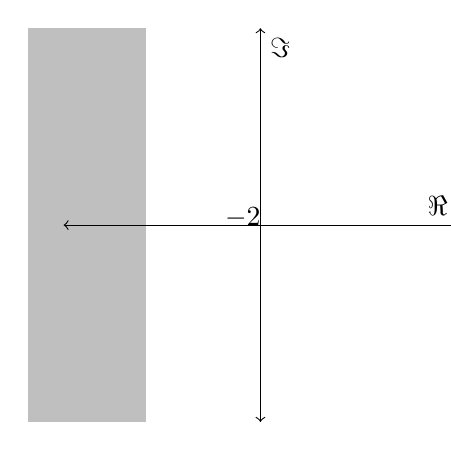
\begin{tikzpicture}
  \path [draw=none,fill=lightgray] (-2.5,-2.5)--(-1,-2.5)--(-1,2.5)--(-2.5,2.5)--cycle;
  \vtick{-1} node[pos=0.5,below] {$-2$};
  \draw [<->] (-2.5,0) -- (2.5,0) node [above left]  {$\Re$};
  \draw [<->] (0,-2.5) -- (0,2.5) node [below right] {$\Im$};
\end{tikzpicture}
\hspace{0.3cm}
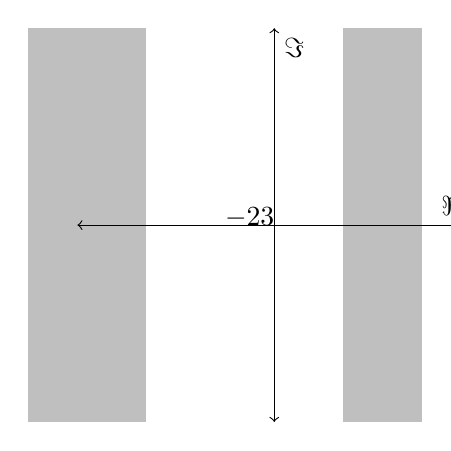
\begin{tikzpicture}
  \path [draw=none,fill=lightgray] (-2.5,-2.5)--(-1,-2.5)--(-1,2.5)--(-2.5,2.5)--cycle;
  \path [draw=none,fill=lightgray] (2.5,2.5)--(1.5,2.5)--(1.5,-2.5)--(2.5,-2.5)--cycle;
  \vtick{-1} node[pos=0.5,below] {$-2$};
  \vtick{1.5} node[pos=0.5,below] {$3$};
  \draw [<->] (-2.5,0) -- (2.5,0) node [above left]  {$\Re$};
  \draw [<->] (0,-2.5) -- (0,2.5) node [below right] {$\Im$};
\end{tikzpicture} 
\\ \vspace{0.3cm}
\begin{tikzpicture}
  %\path [draw=none,fill=lightgray] (-2.5,-2.5)--(-1,-2.5)--(-1,2.5)--(-2.5,2.5)--cycle;
  \vtick{-1} node[pos=0.5,below] {$-2$};
  \draw [<->] (-2.5,0) -- (2.5,0) node [above left]  {$\Re$};
  \draw [<->] (0,-2.5) -- (0,2.5) node [below right] {$\Im$};
\end{tikzpicture}
\;\;\;
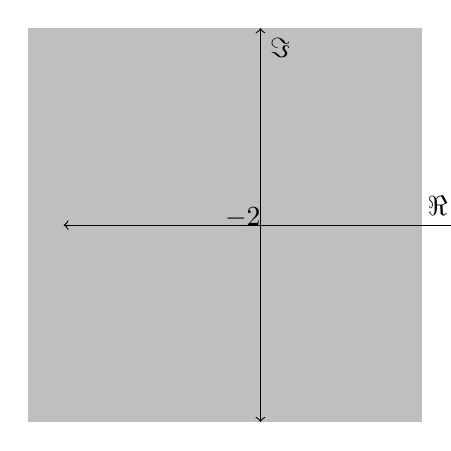
\begin{tikzpicture}
  \path [draw=none,fill=lightgray] (-2.5,-2.5)--(2.5,-2.5)--(2.5,2.5)--(-2.5,2.5)--cycle;
  \vtick{-1} node[pos=0.5,below] {$-2$};
  \draw [<->] (-2.5,0) -- (2.5,0) node [above left]  {$\Re$};
  \draw [<->] (0,-2.5) -- (0,2.5) node [below right] {$\Im$};
\end{tikzpicture}
\caption{Regions of convergence (unshaded) for the signal $e^{-2t} u(t)$ (top left), the signal $e^{-2t}u(t) + e^{3t}u(-t)$ (top right), the rectangular pulse $\Pi$ (bottom left), and the constant signal $x(t) = 1$ (bottom right). }\label{fig:rocexample1}
\end{figure}

%\section{The inverse Laplace transform}

Given the Laplace transform $\calL x \in \roc x \to \complex$ the signal $x$ can be recovered by the \term{inverse Laplace transform}
\[
x(t) = \frac{1}{2\pi j} \lim_{\omega \rightarrow\infty} \int_{\sigma - j\omega}^{\sigma - j\omega} \calL x(s) e^{st} ds,
\]
where $\sigma$ is any real number inside the region of convergence $\roc x$.  Solving the integral above typically requires a special type of integration called \term{contour integration} that we will not consider here~\citep{Stewart_ComplexAnalysis_2004}.  For our purposes, and for many engineering purposes, it suffices to remember only the following Laplace transform pair
\begin{equation}\label{eq:laplacetranscommonsimple}
\calL\big(t^n u(t)\big) = \frac{n!}{s^{n+1}} \qquad \Re(s) > 0,
\end{equation}
where $n \geq 0$ is an integer (Exercise~\ref{excer:laplacetransformcommonpolyut}).  The Laplace transforms of the signal $x(t)$ and the signal $e^{\alpha t}x(t)$ are related,
\begin{align}
\calL\big( e^{\alpha t} x(t)\big)\big(s\big) &= \int_{-\infty}^{\infty} e^{\alpha t} x(t)  e^{-s t} dt \nonumber \\
&= \int_{-\infty}^{\infty} x(t)  e^{-(s-\alpha) t} dt \nonumber \\
&=  \calL x(s-\alpha) \qquad s - \alpha \in \roc x. \label{eq:freqshiftrule}
\end{align}
The region of convergence of $\calL(e^{\alpha t}x(t)\big)$ is all those complex numbers $s$ such that $s - \alpha \in \roc x$.  This is called the \term{frequency-shift rule}.  Combining the frequency-shift rule with~\eqref{eq:laplacetranscommonsimple} we obtain the transform pair
\begin{equation}\label{eq:laplacetneucommon}
\calL\big( t^n e^{\alpha t} u(t) \big) = \frac{n!}{(s-\alpha)^{n+1}} \qquad \Re(s) > \Re(\alpha),
\end{equation}
where $n \geq 0$ is an integer.  This is the only Laplace transform pair we require here.  

A useful relationship exists between the Laplace transform of a signal $x(t)$ and its time-scaled version $x(\alpha t)$ where $\alpha \neq 0$,
\begin{equation}\label{eq:timescalingpropertrylaplacetrans}
 \calL\big(x(\alpha t)\big)\big(s\big) = \frac{1}{\abs{\alpha}}\calL x(s/\alpha), \qquad \Re(s/\alpha) \in \roc x.
\end{equation}
The region of convergence of $\calL\big(x(\alpha t)\big)$ is those complex numbers $s$ such that $s/\alpha \in \roc x$.  This is called the \term{time-scaling property} of the Laplace transform (Excercise~\ref{excer:timescalelaplace}).

 
% Observe that the signal $t^n e^{\alpha t} u(t)$ is right sided.  It is nonzero only when $t > 0$.  The region of convergence is a right half plane $\Re(s) > \alpha$.  The Laplace transform $n!/s^{n+1}$ also corresponds with the left sided signal $(-t)^n e^{-\alpha t} u(-t)$.  That is,
% \[
% \calL\big( (-t)^n e^{-\alpha t} u(-t) \big) = \frac{n!}{(s-\alpha)^{n+1}} \qquad \Re(s) < \alpha,
% \]
% where the region of convergence is now a left half plane.  The practical systems that we analyse in this course are causal, and have right sided impulses responses.  For this reason the left sided signal $(-t)^n e^{-\alpha t} u(-t)$ will not be of significant use.


% For our purposes, and for most engineering purposes, it suffices to obtain inverse Laplace transforms using a table such as Table~\ref{table:laplacetrans}.

% \begin{table}[tp]
% \centering
% \begin{tabular}{lll}
% $x(t)$ & $\calL(x,s)$ & ROC \\ \toprule
% $e^{-\alpha t} u(t)$ & $\frac{1}{s+\alpha}$ & $\Re(s) > -\alpha$ \\ 
% $t e^{-\alpha t} u(t)$ & $\frac{1}{(s+\alpha)^2}$ & $\Re(s) > -\alpha$ \\ 
% $t^n e^{-\alpha t} u(t)$ & $\frac{n!}{(s+\alpha)^{n+1}}$ & $\Re(s) > -\alpha$ \\ 
% %$e^{-\alpha{t}} u(t) \cos(\beta t)$ & $\frac{s + \alpha}{(s+\alpha)^2 + \beta^2}$ & $\Re(s) > -\alpha$ \\
% %$e^{-\alpha{t}} u(t) \sin(\beta t)$ & $\frac{\beta}{(s+\alpha)^2 + \beta^2}$ & $\Re(s) > -\alpha$ \\
% %$e^{-\alpha{t}} u(t) \big( \cos(\beta t) + \gamma\sin(\beta t) \big)$ & $\frac{s + \alpha + \beta\gamma}{(s+\alpha)^2 + \beta^2}$ &  $\Re(s) > -\alpha$ \\ \bottomrule
% \end{tabular}
% \caption{Table of common Laplace transforms and their regions of convergence (ROC).}\label{table:laplacetrans}
% \end{table}


\section{The transfer function and the Laplace transform}\label{sec:transf-funct-lapl}

We have already discovered that the transfer function $\lambda H$ of a regular system $H$ with impulse response $h$ is equal to the Laplace transform $\calL h$ of the impulse response, that is,
\[  
\lambda H(s) = \calL h(s) \qquad s \in \roc h.
\]
The transfer functions of the shifter $T_\tau$ and differentiator $D$ can be obtained by inspection.  For the shifter
\begin{equation}\label{eq:timeshiftertransferfunction}
T_\tau e^{st} = e^{s(t-\tau)} = e^{-s\tau} e^{st} \qquad \text{and so} \qquad \lambda T_\tau = e^{-s\tau}.
\end{equation}
%The region of convergence is the whole complex plane $s \in \complex$.  
For the special case of the identity system $T_0$ we obtain $\lambda T_0 = 1$.  For the differentiator
\[
D e^{st} = \frac{d}{d t} e^{st} = s e^{st} \qquad \text{and so} \qquad \lambda D = s.
\]
%The region of convergence is the whole complex plane $s \in \complex$.  
More generally, for the $k$th differentiator
\begin{equation}\label{eq:lambdadifferentiator}
D^k e^{st} = \frac{d^k}{d t^k} e^{st} = s^k e^{st} \qquad \text{and so} \qquad  \lambda D^k = s^k.
\end{equation}
The domain of $\lambda T_\tau$ and of $\lambda D^k$ is the entire complex plane $\complex$.
%The region of convergence is again the whole complex plane.  
These results motivate assigning the following Laplace transforms to the delta ``function'' $\delta$, its shift $T_\tau \delta = \delta(t - \tau)$, and the $\delta^k$ symbol,
\[
\calL \delta = 1, \qquad \calL\big( \delta(t - \tau) \big) = e^{-s\tau}, \qquad \calL \delta^k = s^k.
\]
These conventions are common in the literature~\citep{Oppenheiim_sigs_sys_1996}.

%\subsection{The transfer function of a linear combination of systems}

Let $F \in X \to Y$ and $G \in X \to Y$ be linear shift-invariant systems with domain $X$ and let $H = a F + bG$ be the system formed by a linear combination of $F$ and $G$.  The response of $H$ to the complex exponential signal $e^{st} \in X$ is
\begin{align*}
H e^{st} &= a F e^{st} + b G e^{st} \\
&= a\lambda F(s) e^{st} + b\lambda G(s) e^{st}  \\
&= \big( a\lambda F(s) + b\lambda G(s) \big) e^{st} \\
&= \lambda H(s)  e^{st}
\end{align*}
and so $\lambda H = a\lambda F + b\lambda G$.  That is, the transfer function of a linear combination of systems is the same linear combination of the transfer functions.  %The region of convergence of the linear combination is the intersection of the regions of convergence of the systems being combined.

Now let $F \in X \to Y$ and $G \in Y \to Z$ be linear shift-invariant systems and suppose that the complex exponential signal $e^{st} \in X$ if $e^{st} \in Y$, that is, $\cep X \subset \cep Y$.  This will be the only case of interest to us.  Let $H \in X \to Z$ be the system formed by the composition $H = G F$.  The response of $H$ to the signal $e^{st} \in X$ satisfies
\[
H e^{st} = G F e^{st} = G \big(\lambda F(s) e^{st} \big) = \lambda F(s) G e^{st}
\]
and since $e^{st}$ is also in $Y$,
\[
H e^{st} = \lambda F(s) \lambda G(s) e^{st} = \lambda H(s) e^{st}.
\]
It follows that
\begin{equation}\label{eq:composedtransferfunction}
\lambda H(s) = \lambda F(s) \lambda G(s) \qquad s \in \cep X = \cep X \cap \cep Y.
\end{equation}
That is, the transfer function of a composition of linear shift-invariant systems is the multiplication of the transfer functions of those systems.  %The region of convergence of the composition is the intersection of the regions of convergence of the systems being composed.

%\subsection{The convolution theorem}

Now suppose that $F$ and $G$ are regular systems with impulse responses $f$ and $g$.  We showed in Section~\ref{sec:line-comb-comp} that the composition $H = G F$ is a regular system with impulse response given by the convolution $h = g * f$ and with domain $\dom f\;g$.  It can be shown that $e^{st} \in \dom f\;g$ if and only if $s \in \roc f \cap \roc g$, that is, $\cep \dom f\;g = \roc f \cap \roc g$ (Exercise~\ref{exer:domfgrocfrocg}).  Thus, for $s \in \roc f \cap \roc g$ we have
\[ 
\lambda H(s) = \calL h(s)  \qquad \lambda F(s) = \calL f(s) \qquad \lambda G(s) = \calL g(s),
\] 
and using~\eqref{eq:composedtransferfunction}, dropping the ``(s)'' for notationial clarity, we obtain,
\[
\calL(f * g) = \calL h =  \lambda H = \lambda F \lambda G = \calL f \calL g
\]
for $s \in \roc f \cap \roc g$.  Putting $x = f$ and $y = g$, we obtain the \term{convolution theorem},
\begin{equation}\label{eq:convtheoremlaplace}
\calL(x*y) = \calL x \calL y
\end{equation}
with region of convergence $\roc x \cap \roc y$.  In words: the Laplace transform of a convolution of signals is the multiplication of their Laplace transforms.  The region of convergence of $\calL(x * y)$ is the intersection of the regions of convergence of $\calL x$ and $\calL y$, that is, $\roc x \cap \roc y$.  
%This is called and goes by the phrase: ``Convolution in the time domain is multiplication in the Laplace/Fourier/Frequency domain''.

%\subsection{The Laplace transform of an output signal}

Let $H$ be a regular system with impulse response $h$ and let $y = H x$ be the response of the system $H$ to input signal $x \in \dom h$.  We have $y = h * x$ and the convolution theorem asserts that
\begin{equation}\label{eq:transferLaplcetheorem}
\calL y = \calL h \calL x = \lambda H \calL x
\end{equation}
with region of convergence $\roc h \cap \roc x$.  Thus, the Laplace transform of the response $y = H x$ is the transfer function of the system regular system $H$ multiplied by the Laplace transform of the input signal $x$.  This result also holds for the shifter, that is,
\[
\calL T_{\tau} x = \lambda T_\tau \calL x = e^{-s\tau} \calL x
\]
with region of convergence is $\roc x$.  This is called the \term{time-shift property} of the Laplace transform (Exercise~\ref{exer:laplacetranstimeshift}).  The result also holds for the differentiator, that is,
\[
\calL D x = \lambda D \calL x = s \calL x
\]
with region of convergence is $\roc x$ under the added assumptions that $x$ is differentiable, i.e. $x \in C^1$, and that the limits $\lim_{t\to\infty} x(t) e^{-st}$ and $\lim_{t\to-\infty} x(t) e^{-st}$ both converge to zero when $s \in \roc x$.  This is called the \term{differentiation property} of the Laplace transform (Exercise~\ref{exer:laplacetransdiffproperty}).  Observe that the assumption is true if, for example, $x(t)$ is finite. %A of signal that does not satisfy the differentiation property is $u(t) \sin(e^{t^2})$.

% \subsection{Commutivity (again)}

% We can now state something about the commutivity of two linear shift-invariant systems $F$ and $G$.  From~\eqref{eq:composedtransferfunction} the composition $F\big(G(x)\big)$ and the composition $G\big(F(x)\big)$ have the same transfer functions and the same regions of convergence $R_1 \cap R_2$.  From~\eqref{eq:transferLaplcetheorem} we have that the Laplace transform of the output signal $y_1 = F\big(G(x)\big)$ and of the output signal $y_2 =G\big(F(\cdot)\big) F\big(G(x)\big)$ satisfy
% \[
% \calL(y_1) = \lambda(F)\lambda(G) = \lambda(G)\lambda(F) = \calL(y_2), \qquad s \in R_1 \cap R_2 \cap R_x.
% \]
% It follows that $y_1 = y_2$ because $\calL(y_1) = \calL(y_2)$ and these signals have the same region of convergence $R_1 \cap R_2 \cap R_x$.  Thus, $F$ and $G$ commute for all input signal $x$ with region of convergence $R_x$ intersecting $R_1 \cap R_2$, i.e., such that $R_1 \cap R_2 \cap R_x \neq \emptyset$.

% \begin{theorem}\label{thm:laplacetranslti}
% Let $H$ be a linear shift-invariant system and let $y$ be the reponse of $H$ to intput signal $x$, that is $y = H(x)$.  The Laplace transforms of $x$ and $y$ are related by
% \[
% \calL(y,s) = \lambda(H,s) \calL(x,s),
% \]
% for all $s$ such that $\calL(x,s)$ and $\lambda(H,s)$ exist.
% \end{theorem}
% \begin{proof}
% We present a proof only for the case that $H$ is a regular system with impulse response $h$.  One can check that the result also holds for differentiators and time shifters.  Taking the Laplace tranform of $y$ gives
% \begin{align*}
% \calL(y,s) &= \calL(H(x),s) \\
% &= \int_{-\infty}^{\infty} H(x,t) e^{-st} dt \\
% &= \int_{-\infty}^{\infty} \int_{-\infty}^{\infty} h(\tau) x(t - \tau)  e^{-st}  d\tau dt
% \end{align*}
% and by a change of variable $\kappa = t - \tau$,
% \begin{align*}
% \calL(y,s) &=  \int_{-\infty}^{\infty} \int_{-\infty}^{\infty} h(\tau) x(\kappa) e^{-s(\kappa+\tau)} d\tau d\kappa \\
% &= \int_{-\infty}^{\infty} x(\kappa) e^{-s\kappa} \int_{-\infty}^{\infty} h(\tau) e^{-s\tau} d\tau d\kappa.
% \end{align*}
% Observe that
% \[
% \lambda(H,s) = \int_{-\infty}^{\infty} h(\tau) e^{-s\tau} d\tau
% \]
% is the transfer function of $H$, and so
% \begin{align*}
% \calL(y,s) &= \int_{-\infty}^{\infty} x(\kappa) e^{-s\kappa} \lambda(H,s) d\kappa \\
% &= \lambda(H,s) \int_{-\infty}^{\infty} x(\kappa) e^{-s\kappa} d\kappa \\
% &= \lambda(H,s) \calL(x,s).
% \end{align*}
% \end{proof}

% \begin{proof} (Sketch) Taking the Laplace tranform of $y$ gives
% \[
% \calL(y,s) = \calL(H(x),s) = \int_{-\infty}^{\infty} H(x,t) e^{-st} dt,
% \]
% and by a change of variable $\kappa = t - \tau$,
% \begin{align*}
% \calL(y,s) &=  \int_{-\infty}^{\infty} H(x,\kappa+\tau) e^{-s(\kappa+\tau)} d\kappa \\
% &= e^{-s\tau} \int_{-\infty}^{\infty} H(x,\kappa+\tau) e^{-s\kappa} d\kappa.
% \end{align*}
% Because $H$ is shift-invariant we have, using~\eqref{eq:timeinvvarchange},
% \[
% H(x,\kappa+\tau) = H(T_{-\kappa}(x),\tau),
% \]
% and so
% \[
% \calL(y,s) = e^{-s\tau} \int_{-\infty}^{\infty} H(T_{-\kappa}(x),\tau) e^{-s\kappa} d\kappa.
% \]
% Under the conditions imposed by the theorem we can move the integral inside the system $H$ to obtain 
% \begin{equation}\label{eq:Hwithathm1}
% \calL(y,s) = e^{-s\tau} H( z ,\tau)
% \end{equation}
% where $z$ is the signal
% \begin{align*}
% z(\tau) = \int_{-\infty}^{\infty} T_{-\kappa}(x,\tau) e^{-s\kappa} d\kappa = \int_{-\infty}^{\infty} x(\kappa+\tau) e^{-s\kappa} d\kappa.
% \end{align*}
% By the change of variables $t = \kappa + \tau$,
% \[
% z(\tau) = \int_{-\infty}^{\infty} x(t) e^{-s(t - \tau)} d\kappa = e^{s\tau} \calL(x,s).
% \]
% Substituting this into~\eqref{eq:Hwithathm1} gives
% \[
% \calL(y,s) = e^{-s\tau} H( e^{s\tau} \calL(x,s) ,\tau) = e^{-s\tau} \calL(x,s) H( e^{s\tau} ,\tau)
% \]
% since $\calL(x,s)$ does not depend on $\tau$.  By definition $H( e^{s\tau} ,\tau) = e^{s\tau} \lambda(H,s)$ and we immediately have $\calL(y,s) = \calL(x,s) \lambda(H,s)$ as required.
% \end{proof}

% If the Laplace transform of a signal $x$ exists then 
% \begin{equation}\label{eq:laplacelimits}
% \lim_{t\rightarrow\infty} x(t)  e^{-st} = 0 \qquad \text{and}  \lim_{t\rightarrow-\infty} x(t)  e^{-st} = 0,
% \end{equation}
% as otherwise the integral~\ref{eq:laplace_defn} defining $\calL(x)$ would not exists.

% Let $x$ be a differentiable signal with Laplace transform $\calL(x)$.  The Laplace transform of the derivative $\frac{d}{dt}x$ of $x$ is
% \begin{align*}
% \calL\left( \frac{d}{dt}x \right) &= \int_{-\infty}^{\infty}  \left(\frac{d}{dt} x(t)\right)  e^{-st}  dt \\
% &= \int_{-\infty}^{\infty}  \frac{d}{dt} \big( x(t)  e^{-st} \big)  + s x(t) e^{-st}  dt \\
% &= \int_{-\infty}^{\infty}  \frac{d}{dt} \big( x(t)  e^{-st} \big)  dt + s \int_{-\infty}^{\infty}  x(t) e^{-st}  dt \\
% &=  s \calL(x),
% \end{align*}
% the second line following from the product rule for differentiation,
% \begin{align*}
% \frac{d}{dt} \big( x(t)  e^{-st} \big) &= \left(\frac{d}{dt} x(t)\right)  e^{-st} + x(t) \frac{d}{dt}e^{-st} \\
% &= \left(\frac{d}{dt} x(t)\right) e^{-st} - s x(t) e^{-st},
% \end{align*}
% the last line since $\calL(x) = \int_{-\infty}^{\infty}  x(t) e^{-st}dt$ is the Laplace transform of $x$ and because
% \[
% \int_{-\infty}^{\infty}  \frac{d}{dt} \big( x(t)  e^{-st} \big) = \lim_{t\rightarrow\infty} x(t)  e^{-st} - \lim_{t\rightarrow-\infty} x(t)  e^{-st} = 0
% \]
% by the fundamental theorem of calculus and~\eqref{eq:laplacelimits}.


%section{Solving differential equations}\label{sec:solv-diff-equat}

In Chapter~\ref{sec:syst-modell-diff} we modelled electrical, mechanical, and electromechanical devices by linear differential equations with constant coefficients of the form
\[
\sum_{\ell=0}^{m} a_\ell D^\ell x = \sum_{\ell=0}^{k} b_\ell D^\ell y.
\]
Suppose that $H$ is a linear shift-invariant system such that $y = Hx$ if $x$ and $y$ satisfy a differential equation of this form.  In Section~\ref{sec:eigenf-line-time} we found that the transfer function of $H$ is a ratio of polynomials, that is,
\[
\lambda H(s) = \frac{\sum_{\ell=0}^{m} a_\ell s^{\ell} e^{st}}{\sum_{\ell=0}^{k} b_\ell s^{\ell} e^{st}} = \frac{a_0 + a_1s + \dots a_m s^m}{b_0 + b_1s + \dots b_k s^k}.
\]
Properties of $H$ can be obtained by inspecting this transfer function.  For example, the impulse response of $H$ (if it exists) can be obtained by applying the inverse Laplace transform.

We now apply these results to the differential equations that model the RC electrical circuit from Figure~\ref{circ:seriesRC1} and the mass spring damper from Figure~\ref{mech:massspring1}.  The RC circuit is an example of what is called a \term{first order system} and the mass spring damper is an example of what is called a \term{second order system}.

\section{First order systems}\label{sec:first-order-systems}

Recall the passive electrical RC circuit from Figure~\ref{circ:seriesRC1}.  The differential equation modelling this circuit is~\eqref{eq:diffequform},
\[
x = y + RC D y
\] 
where $x$ is the input voltage signal, $y$ is the voltage over the capacitor, and $R$ and $C$ are the resistance and capacitance.  The RC circuit is an example of a \term{first order system} so called because the highest order derivative that occurs is of order one, that is, $D^k$ with $k = 1$.  Let $H$ be a system mapping the input voltage signal $x$ to the output voltage signal $y$.  From~\eqref{eq:findtransferfuncfromdiff} the transfer function $\lambda H$ is found to satisfy
\[
\lambda H(s) = \frac{1}{1 + RC s} = \frac{r}{r + s}
\]
where $r = \tfrac{1}{RC}$.  The value $\tfrac{1}{r} = RC$ is called the \term{time constant}.  The impulse response of $H$ is given by the inverse of this Laplace transform.  There are two signals with Laplace transform $\frac{r}{r + s}$: the right sided signal $r e^{-r t} u(t)$ with region of convergence $\Re(s) > -r$, and the left sided signal $-r e^{-r t} u(-t)$ with region of convergence $\Re(s) < -r$.  The RC circuit (and in fact all physically realisable systems) are expected to be causal.  For this reason, the left sided signal $ -r e^{-r t} u(-t)$ cannot be the impulse response of $H$.  The impulse response is the right sided signal
\[
h(t) = r e^{-r t} u(t).
\]
%Figure~\ref{fig:firstorderresponsesstableunstable} plots this impulse response for an RC circuit with $r = \frac{1}{RC} = -\tfrac{1}{5}, 1, \tfrac{1}{5}$.  
Given an input voltage signal $x$ we can now find the corresponding output signal $y = Hx$ by convolving $x$ with the impulse response $h$.  That is,
\[
y = Hx = h * x = \int_{-\infty}^{\infty} r e^{-r \tau} u(\tau) x(t - \tau) d\tau = r \int_{0}^{\infty} e^{-r \tau} x(t - \tau) d\tau.
\] 
%The output signal $y$ exists whenever this convolution exists.  The domain of $H$ is the set of input signals $x$ such that the convolution $h * x$ does exist. 

If $r \geq 0$ the impulse response is absolutely integrable, that is,
\begin{align*}
\|h\|_1 &= \int_{-\infty}^\infty \abs{r e^{-r t} u(t)} dt \\
&= r \int_{0}^\infty e^{-r t} dt \\
&= 1 - \lim_{t\to\infty} e^{-r t} = 1,
\end{align*}
and the system is stable (Exercise~\ref{excer:bibostableimpulseresp}).  However, if $r < 0$ the impulse response is not absolutely integrable and the system is not stable.  Figure~\ref{fig:firstorderresponsesstableunstable} shows the impulse response when $r=-\frac{1}{5}, -\tfrac{1}{3}, -\tfrac{1}{2}, 1, 2$.  In a passive electrical RC circuit the resistance $R$ and capacitance $C$ are always positive and $r=\tfrac{1}{RC}$ is positive. For this reason, passive electrical RC circuits are always stable.

From~\eqref{eq:stepresponseintegrateimpulseresponse}, the step response $Hu$ is given by applying the integrator $I_\infty$ to the impulse response, that is, 
\[
Hu = I_\infty h = \int_{-\infty}^t r e^{-r \tau} u(\tau) d\tau =  \begin{cases}
r \int_{0}^t e^{-r \tau} d\tau & t > 0 \\
0 & \text{otherwise} 
\end{cases}
\]
or more simply
\begin{equation}\label{eq:stepresponsefirstorder}
Hu = \big( 1 - e^{-r t}\big) u(t).
\end{equation}
This step response in plotted in Figure~\ref{fig:firstorderresponsesstableunstable}.

% We can also discover the output signal $y$ given a specific input signal $x$.  For example, consider 
% \[
% x(t) = \rect\big(t-\tfrac{1}{2}\big) = \begin{cases}
% 1 & 0 < t \leq 1\\
% 0 & \text{otherwise},
% \end{cases}
% \]
% where $\rect(t)$ is the rectangular pulse~\eqref{eq:rectfuncdefn}.  The Laplace transform of $x$ is, 
% \begin{align*}
% \calL(x) = \int_{-\infty}^{\infty} x(t) e^{-st} dt = \int_{0}^{1} e^{-st} dt = \frac{1  - e^{-s}}{s},
% \end{align*}
% and so, Laplace transform of $y$ is
% \[
% \calL(y) = \frac{\tau}{\tau + s} \calL(x) = \tau\frac{1 - e^{-s}}{s(\tau + s)}.
% \]
% Since $e^{-s}$ is the transfer function of the time shifter $T_{1}$,
% \[
% y =  g - T_{1}(g) = g(t) - g(t - 1),
% \]
% where $g$ is the signal with Laplace transform
% \[
% \calL(g) = \frac{\tau}{s(\tau + s)}.
% \]
% Applying partial fractions we obtain
% \[
% \calL(g) = \frac{1}{s} - \frac{1}{\tau + s}.
% \]
% Using~\eqref{eq:laplacetneucommon} we obtain the transform pairs
% \[
% \calL\big(u(t)\big) = \frac{1}{s}, \qquad \calL\big(e^{-st}u(t)\big) = \frac{1}{\tau + s}
% \]
% and so $g(t) = u(t)( 1 - e^{-\tau t})$, and
% \[
% p(t) = u(t)( 1 - e^{-\tau t}) - u(t-1)( 1 - e^{-\tau (t-1)}).
% \]
% This response is plotted on the right hand side of Figure~\ref{fig:firstorderresponses}.



%\begin{randomfloat}
\begin{test}\label{test:activeRCtestagain} 
(\textbf{The impulse response of the active RC circuit})
In this test we again use the active RC circuit from Test~\ref{test:activeRCtest} with resistors $R=R_1=R_2=27\si{\kilo\ohm}$ and capacitor $C=C_2=10\si{\nano\farad}$.  In Test~\ref{test:activeRCtest} we applied the differential equation~\eqref{eq:activeRC} to the reconstructed output signal $\tilde{y}$ and asserted that the resulting signal was close to the reconstructed input signal $\tilde{x}$.  In this test we instead convolve the input signal $\tilde{x}$ with the impulse response 
\[
h(t) = -\tfrac{1}{RC} e^{-t/RC}u(t) = -r e^{-rt}u(t), \qquad r = \tfrac{1}{RC} = \frac{10^5}{27}
\] 
and assert that the resulting signal is close to the output signal $\tilde{y}$.  That is, we test the expected relationship
\[
\tilde{y} \approx h * \tilde{x} = \int_{-\infty}^\infty h(\tau) \tilde{x}(t - \tau) d\tau.
\]
From~\eqref{eq:xreconstruct},
\begin{align*}
\tilde{y}(t) &\approx  \int_{-\infty}^{\infty} h(\tau) \sum_{\ell=1}^L x_\ell \sinc( Ft - F\tau - \ell ) d\tau \\
&= \sum_{\ell=1}^L  x_\ell \int_{-\infty}^{\infty} h(\tau) \sinc( Ft - F\tau - \ell ) d\tau \\
&= \sum_{\ell=1}^L  x_\ell g( Ft - \ell )
\end{align*}
where the function
\[
g(t) = \int_{-\infty}^\infty h(\tau) \sinc( t - F\tau ) d\tau = -r \int_{0}^\infty e^{-r\tau} \sinc( t - F\tau ) d\tau.
\]
% It is helpful to transform $g(t)$ into the form more ammenable to numerical integration
% \[
% g(t) = -\int_{-\pi}^{\pi} \frac{\cos(\omega t ) + V^2 \omega t \sin(\omega t )}{1 + \omega^2t^2} \; d\omega \qquad \text{(Exercise~\ref{?})}
% \]
% where $V = \tfrac{F}{r} = $.  
% We will make a numerical approximation of $g(t)$.  It is helpful to first make the change of variable $k = r \tau$ so that
% \[
% g(t) = \int_{0}^\infty e^{-k} \sinc( t - Vk ) dk
% \]
% where $V = \tfrac{F}{r} = \tfrac{11907}{1000}$. First observe that $g(t)$ small values when $\abs{t}$ is large, specifically,
% \[
% \abs{g(t)} \leq \int_{0}^\infty e^{-k} \abs{\sinc( t - Vk )} dk \leq  \frac{1}{\abs{t}} \int_{0}^\infty \tfrac{ e^{-k}} = \frac{e}{\abs{t}}
% \]
% and so, we will approximate $g(t)$ by zero when $\abs{t} > T = 10^3$.  This approximation is accurate to 3 decimal places. For $\abs{t} < 10^3$ we truncate the upper bound of the integral,
% \[
% g(t) \approx \int_{0}^{B} e^{-k} \sinc( t - Vk ) dk
% \] 
% where $B$ is chosen so that 
% \[
% \abs{\int_{0}^{B} e^{-k} \sinc( t - Vk ) dk} \leq \frac{1}{\abs{t}} \int_{0}^{B} e^{-k} dk = 
% \]
An approximation of $g(t)$ is made by the trapezoidal sum
\[
g(t) \approx \frac{K}{2N} \left( p(0) + p(K) + 2 \sum_{n=1}^{N-1} p( \Delta n ) \right),
\]
where $p(\tau) = h(\tau) \sinc( t - F\tau )$ and
\[
K = -RC\log\big(10^{-3}\big), \qquad N = \ceil{10 F K}, \qquad \Delta = K/N.
\]
Figure~\ref{fig:test:activeRCagain} plots the input signal $\tilde{x}$, output signal $\tilde{y}$, and hypothesised output signal $h * \tilde{x}$ over a $4\si{\milli\second}$ window.

\begin{center}
  \begin{tikzpicture}
    \selectcolormodel{gray} 
    \begin{axis}[compat=newest,font=\footnotesize,height=8cm,width=12cm,xlabel={time (s)},ylabel={electrical potential}, legend style={draw=none,fill=none,legend pos=north west,cells={anchor=west},font=\footnotesize},xmin=999.92,xmax=1004.08,ytick={0}, yticklabels={0},xtick={1000,1001,1002,1003,1004},xticklabels={1.000,1.001,1.002,1.003,1.004}]
      \addplot[mark=none] table[x index=0, y index=1] {tests/activeRC/data.csv};
      \addplot[mark=o,mark repeat=10,mark options={solid,fill=black,scale=1.1}] table[x index=0, y index=2] {tests/activeRCagain/data.csv};
      \addplot[mark=*,mark repeat=10,mark options={solid,fill=black,scale=0.6}] table[x index=0, y index=3] {tests/activeRCagain/data.csv};
      \legend{$\tilde{x}$, $\tilde{y}$, $h*\tilde{x}$ }
   \end{axis} 
  \end{tikzpicture}
\captionsetup{type=figure}
%\includegraphics{tests/activeRCagain/plot-1.mps}
\captionof{figure}{Plot of reconstructed input signal $\tilde{x}$ (solid line), output signal $\tilde{y}$ (solid line with circle), and hypothesised output signal $h * \tilde{x}$ (solid line with dot).}\label{fig:test:activeRCagain}
\end{center}
\end{test}
%\end{randomfloat}


\begin{figure}[tp]
\centering

\begin{tikzpicture}[domain=0:5,samples=100]
  \begin{scope}[scale=2]
    \draw[->] (-0.5,0) -- (5.25,0) node[above] {$t$};
    \draw[->] (0,-1.5) -- (0,2.25) node[right] {$h$};
    \draw[thick] (-0.25,0) -- (0,0) -- (0,2);
    \draw[thick] (0,0) -- (0,-1/2);
    % \draw[color=black,thick,samples=100,domain=0:4] plot function{-exp(x/5)/5};
    \begin{scope}
      \clip (-0.2,-1.25) rectangle (10.5,2.1);
      % \draw[color=black,thick] plot function{-exp(x/8)/8};
      \draw[color=black,thick] plot function{-exp(x/5)/5};
      \draw[color=black,thick,domain=0:4] plot function{-exp(x/2)/2};
      \draw[color=black,thick,domain=0:6] plot function{-exp(x/3)/3};
      \draw[color=black,thick] plot function{exp(-x)};
      \draw[color=black,thick] plot function{2*exp(-2*x)};
      \draw[color=black,thick] plot function{exp(-x/2)/2};
    \end{scope}
     \begin{scope}[font=\small]
       \node[right] at (0.2,1.4) {$2$};
       \node[right] at (0.15,0.9) {$1$};
       \node[right] at (0.2,0.3) {$\tfrac{1}{2}$};
       \node at (1,-1) {$-\tfrac{1}{2}$};
       \node at (2.7,-1) {$-\tfrac{1}{3}$};
       \node at (4,-0.6) {$-\tfrac{1}{5}$};
     \end{scope}
  \end{scope}
  \htick{2} node[pos=0.5,left] {$1$};
  \htick{4} node[pos=0.5,left] {$2$};
  \htick{-2} node[pos=0.5,left] {$-1$};
  \vtick{2} node[pos=0.5,below] {$1$};
  \vtick{4} node[pos=0.5,below] {$2$};
  \vtick{6} node[pos=0.5,below] {$3$};
  \vtick{8} node[pos=0.5,below] {$4$};
  \vtick{10} node[pos=0.5,below] {$5$};
\end{tikzpicture}

\vspace{0.5cm}

\begin{tikzpicture}[domain=0:5,samples=100]
  \begin{scope}[yscale=2,xscale=2]
    \draw[->] (-0.5,0) -- (5.25,0) node[above] {$t$};
    \draw[->] (0,-1.25) -- (0,1.25) node[right] {$H(u)$};
    \draw[thick] (-0.25,0) -- (0,0);
    % \draw[color=black,thick,samples=100,domain=0:4] plot function{1 - exp(x)};
    \begin{scope}
      \clip (-0.2,-1) rectangle (10.5,1.2);
      \draw[color=black,thick] plot function{1 - exp(x/8)};
      \draw[color=black,thick] plot function{1 - exp(x/4)};
      \draw[color=black,thick] plot function{1 - exp(x/2)};
      \draw[color=black,thick] plot function{1 - exp(-2*x)};
      \draw[color=black,thick] plot function{1 - exp(-x/2)};
      \draw[color=black,thick] plot function{1 - exp(-x/4)};  
    \end{scope}
     \begin{scope}[font=\small]
       \node at (0.5,0.75) {$2$};
       \node at (1,0.55) {$\tfrac{1}{2}$};
       \node at (2.5,0.3) {$\tfrac{1}{4}$};
       \node at (0.95,-0.8) {$-\tfrac{1}{2}$};
       \node at (2,-0.8) {$-\tfrac{1}{4}$};
       \node at (3.1,-0.65) {$-\tfrac{1}{8}$};
     \end{scope}
  \end{scope}
  \htick{2} node[pos=0.5,left] {$1$};
  \htick{-2} node[pos=0.5,left] {$-1$};
  %\vtick{2} node[pos=0.5,below] {$1$};
  \vtick{4} node[pos=0.5,below] {$2$};
  \vtick{6} node[pos=0.5,below] {$3$};
  \vtick{8} node[pos=0.5,below] {$4$};
  \vtick{10} node[pos=0.5,below] {$5$};
\end{tikzpicture}

\caption{Top: impulse response of a first order system with $r = -\tfrac{1}{2}$, $-\tfrac{1}{3}$, $-\tfrac{1}{5}$, $\tfrac{1}{2}$, $1$, $2$.  Bottom: step response of a first order system with $r = -\tfrac{1}{2}$, $-\tfrac{1}{4}$, $-\tfrac{1}{8}$, $\tfrac{1}{4}$, $\tfrac{1}{2}$, $2$.}\label{fig:firstorderresponsesstableunstable}
\end{figure}


\section{Second order systems}\label{sec:second-order-systems}

Consider the mass spring damper system from Figure~\ref{mech:massspring1} that is described by the equation
\begin{equation}\label{eq:masspringeqseclapltrans}
f = K p + B D p + M D^2 p
\end{equation}
where $f$ is the force applied to the mass $M$ and $p$ is the position of the mass and $K$ and $B$ are the spring and damping coefficients.  The mass spring damper is an example of a \term{second order system} because it contains differeniators $D^2$ of order at most two.  Another example of a second order system is the Sallen-Key active electrical circuit depicted in Figure~\ref{elec:sallenkey}.  In Section~\ref{sec:syst-modell-diff} we were able to find the force $f$ corresponding with a given position signal $p$.  Suppose that $H$ is a linear shift-invariant system mapping $f$ to $p$, that is, such that $p = Hf$.  We will find the impulse response of $H$.  From~\ref{eq:findtransferfuncfromdiff} the transfer function is found to satisfy
\[
\lambda H(s) =  \frac{1}{K + B s + M s^2}.
\]
We can invert this Laplace transform to obtain the impulse response.  There are three cases to consider depending on whether the quadratic $K + Bs + Ms^2$ has two distinct real roots, is irreducible (does not have real roots), or has two identical real roots.

\paragraph{Case 1: (Distinct real roots)}
In this case, the roots are
\[
\beta-\alpha, \qquad  -\beta-\alpha,
\] 
where 
\[
\alpha = \frac{B}{2M}, \qquad  \beta = \frac{\sqrt{B^2 - 4KM}}{2M}
\]
and $B^2 - 4KM > 0$.  By a partial fraction expansion (Exercise~\ref{exer:partialfracsecondorder}),
\begin{align*}
\lambda H(s) &= \frac{1}{M(s - \beta+\alpha)(s + \beta + \alpha)} \\
&= \frac{1}{2\beta M}\left( \frac{1}{s-\beta+\alpha} - \frac{1}{s+\beta+\alpha} \right).
\end{align*}
From~\eqref{eq:laplacetneucommon} we obtain the transform pairs
\[
\calL(e^{(\beta-\alpha)t} u(t)) = \frac{1}{s-\beta+\alpha}, \qquad \calL(e^{-(\beta+\alpha) t} u(t)) = \frac{1}{s+\beta+\alpha}.
\]
As in Section~\ref{sec:first-order-systems}, other signals with these Laplace transforms are discarded because they do not lead to an impulse response that is zero for $t < 0$.  That is, they do not lead to a causal system $H$.  The impulse response of $H$ is thus
\[
h(t) = \frac{1}{2 \beta M} u(t) e^{-\alpha t} \big( e^{\beta t} - e^{-\beta t} \big).
\]
This is a sum of the impulse responses of two first order systems.

\paragraph{Case 2: (Distinct imaginary roots)}
The solution is as in the previous case, but now $4KM - B^2 > 0$ and $\beta$ is imaginary.  Put $\theta = \beta/j$ so that
\[
e^{\beta t} - e^{-\beta t} = e^{j \theta t} - e^{-j \theta t} = 2 j \sin(\theta t).
\]
The impulse response of $H$ is
\[
h(t) = \frac{1}{ \theta M} u(t) e^{-\alpha t} \sin(\theta t).
\]

\paragraph{Case 3: (Identical roots)}
In this case, the two roots are equal to $-\alpha$ and
\[
\lambda H(s) = \frac{1}{M(s + \alpha)^2}.
\]
From~\eqref{eq:laplacetneucommon} we obtain the transform pair
\[
\calL\big(t e^{-\alpha t} u(t)\big) = \frac{1}{(s + \alpha)^2}
\]
and this is the only signal with this Laplace transform that leads to a causal impulse response.  The impulse response of $H$ is thus
\[
h(t) = \frac{1}{M} t e^{-\alpha t} u(t).
\]

A second order system is called \term{overdamped} when there are two distinct real roots, \term{underdamped} when their are two distinct imaginary roots, and \term{critically damped} when the roots are identical.  The different types of impulse responses for are plotted in Figure~\ref{fig:masspringdamperoscillatory}.

With no damping (i.e. damping coefficient $B = 0$) the roots are of the form $\pm \beta$ and have no real part.  In this case, the impulse response is
\[
h(t) = \frac{1}{ \theta M} u(t) \sin(\theta t),
\]
where $\theta = \beta/j = \sqrt{KM}$ is called the \term{natural frequency} of the second order system.  This impulse response oscillates for all $t > 0$ without decay or explosion.  Two identical roots occur when the damping coefficient $B = \sqrt{4KM}$ and this is sometimes called the \term{critical damping coefficient}.

The impulse response of a second order system is absolutely integrable when $\alpha =  \tfrac{B}{2M} > 0$, but not when $\alpha \leq 0$.  Thus, the system is stable when $\alpha > 0$ and not stable when $\alpha \leq 0$.   For the mass spring damper both the mass $M$ and damping coefficient $B$ are positive and so mass spring dampers are always stable.

From~\eqref{eq:stepresponseintegrateimpulseresponse} the step response $H(u)$ is given by applying the integrator $I_\infty$ to the impulse response.  There are three cases to consider depending on whether the system is overdamped, underdamped, or critically damped.  When the system is overdamped the step response is
\begin{align*}
Hu = I_\infty h &= \frac{1}{2 \beta M} \int_{-\infty}^t e^{-\alpha \tau} \big( e^{\beta \tau} - e^{-\beta \tau} \big) u(\tau) d\tau \\
&= \frac{1}{2 \beta M} \int_{0}^t e^{-\alpha \tau} \big( e^{\beta \tau} - e^{-\beta \tau} \big) d\tau \\
&= \frac{1}{2 \beta M}u(t)\left( \frac{e^{(\beta-\alpha)t}- 1}{ \beta-\alpha} + \frac{e^{-(\beta+\alpha)t}- 1}{\beta+\alpha}\right).
\end{align*}
When the system is underdamped the step response is
\begin{align*}
Hu = I_\infty h &= \frac{1}{ \theta M} \int_{0}^t e^{-\alpha \tau} \sin(\theta \tau) dt \\
&= u(t) \left(\frac{\theta - e^{-t \alpha } \big(\theta  \cos(t \theta)+\alpha  \sin(t \theta)\big)}{M \theta(\alpha ^2+\theta ^2)} \right).
\end{align*}
When the system is critically damped the step response is
\begin{align*}
Hu = I_\infty h &= \frac{1}{ \theta M} \int_{0}^t \frac{1}{M} t e^{-\alpha t} dt \\
&= \frac{1}{M\alpha^2}u(t)\big(1 - e^{-t\alpha s}(1+t\alpha) \big).
\end{align*}
These step responses are plotted in Figure~\ref{fig:masspringdamperoscillatorystepresp}.

\begin{figure}[p]
\centering
\defaultanimation{tikzfigs/impulseresponsemasspringdamper}
%\animategraphics[autoplay,loop,every=\every]{\defaultframerate}{tikzfigs/impulseresponsemasspringdamper}{}{}
\caption{Impulse response of the mass spring damper with $M=1$, $K=\frac{\pi^2}{4}$ and damping constant $B=\tfrac{\pi}{3}$ (underdamped), $B = \sqrt{4KM} = \pi$ (critically damped), and $B = 2\pi$ (overdamped).} \label{fig:masspringdamperoscillatory}
\end{figure}

\begin{figure}[p]
\centering
\defaultanimation{tikzfigs/stepresponsemassspringdamper}
%\animategraphics[autoplay,loop,every=\every]{\defaultframerate}{tikzfigs/stepresponsemassspringdamper}{}{}
\caption{Step response of the mass spring damper with $M=1$, $K=\frac{\pi^2}{4}$ and damping constant $B=\tfrac{\pi}{3}$ (underdamped), $B = \sqrt{4KM} = \pi$ (critically damped), and $B = 2\pi$ (overdamped).} \label{fig:masspringdamperoscillatorystepresp}
\end{figure}


\section{Poles, zeros, and stability}\label{sec:poles-zeros-stab}

The transfer function of a system described by a linear differential equation with constant coefficients is of the form of~\eqref{eq:findtransferfuncfromdiff}, that is,
\[
\lambda H(s) = \frac{a_0 + a_1s + \dots a_m s^m}{b_0 + b_1s + \dots b_k s^k}.
\]
Factorising the polynomials on the numerator and denominator we obtain
\[
\lambda H(s) = C\frac{(s-\alpha_0)(s - \alpha_1)\cdots(s - \alpha_m)}{(s-\beta_0)(s - \beta_1)\cdots(s - \beta_k)},
\] 
where $\alpha_0, \dots, \alpha_m$ are the roots of the numerator polynomial $a_0 + a_1s + \dots + a_m s^m$, and $\beta_0, \dots, \beta_k$ are the roots of the denominator polynomial $b_0 + b_1s + \dots + b_k s^k$, and $C = \tfrac{a_m}{b_m}$.  That such a factorisation is always possible is called the \term{fundamental theorem of algebra}~\citep{Fine_fundamental_theorem_of_algebra}.  %,Weierstraß_fundamental_theorem_of_algebra}.  
If the numerator and denominator polynomials share one or more roots, then these roots cancel leaving the simpler expression
\begin{equation}\label{eq:transfuncpoleszeros}
\lambda H(s) = C\frac{(s-\alpha_d)(s - \alpha_{d+1})\cdots(s - \alpha_{m})}{(s-\beta_d)(s - \beta_{d+1})\cdots(s - \beta_{k})},
\end{equation}
where $d$ is the number of shared roots, these shared roots being 
\[
\alpha_0 = \beta_0, \;\; \alpha_1 = \beta_1, \;\; \dots, \;\;  \alpha_{d-1} = \beta_{d-1}.
\]
%For simplicity in what follows we will assume that there are no shared roots, that is $d = 0$.
The roots from the numerator $\alpha_d, \dots, \alpha_m$ are called the \term{zeros} and the roots from the denominator $\beta_d, \dots, \beta_m$ are called the \term{poles}.  A \term{pole-zero plot} is constructed by marking the complex plane with a cross at the location of each pole and a circle at the location of each zero.  Pole-zero plots for the first order system from Section~\ref{sec:first-order-systems}, the second order system from Section~\ref{sec:second-order-systems}, and the system describing the PID controller~\eqref{eq:PIDdiffeq} are shown in Figure~\ref{fig:polezeroplot}.

\begin{figure}[tp]
  \centering
  \begin{tikzpicture}
    % \path [draw=none,fill=lightgray] (-2.5,-2.5)--(-1,-2.5)--(-1,2.5)--(-2.5,2.5)--cycle;
    % \vtick{-1} node[pos=0.5,below] {$-2$};
    \poletikz{-1}{0} \node[below] at (-1,0) {$-1$};
    \polezeroaxis{2.8}
  \end{tikzpicture}
  \;\;\;
  \begin{tikzpicture}
    \poletikz{-1}{0} \node[below] at (-1,0) {$-1$};
    \poletikz{-2}{0} \node[below] at (-2,0) {$-2$};
    \polezeroaxis{2.8}
  \end{tikzpicture} 
  \\ \vspace{0.3cm}
  \begin{tikzpicture}
    \poletikz{-1}{-2} %\node[below] at (-1,-2) {$-1-2j$};
    \poletikz{-1}{2} %\node[below] at (-1,2) {$-1+2j$};
    \htick{2} node[pos=0.5,right] {$2$};
    \htick{-2} node[pos=0.5,right] {$-2$};
    \vtick{-1} node[pos=0.5,below] {$-1$};
    \polezeroaxis{2.8}
  \end{tikzpicture}
  \;\;\;
  \begin{tikzpicture}
    \poletikz{0}{0} %\node[below] at (-1,0) {$-1-2j$};
    \zerotikz{1}{2} %\node[below] at (1,2) {$1+2j$};
    \zerotikz{1}{-2} %\node[below] at (1,-2) {$1-2j$};
    \htick{2} node[pos=0.5,right] {$2$};
    \htick{-2} node[pos=0.5,right] {$-2$};
    \vtick{1} node[pos=0.5,below] {$1$};
    \polezeroaxis{2.8}
  \end{tikzpicture}
  \caption{Top left: pole zero plot for the first order system $x = y + D y$.  There is a single pole at $-1$. Top right: pole zero plot for the overdamped second order system $x = 2y + 3D y + D^2 y$ that has two real poles at $-1$ and $-2$. Bottom left: pole zero plot for the underdamped second order system $x = 5y + 2 D y + D^2y$ that has two imaginary poles at $-1+2j$ and $-1-2j$.  The poles form a conjugate pair.  Bottom right: pole zero plot for the equation $Dy =  5 x - 2 Dx + D^2x$ that models a PID controller~\eqref{eq:PIDdiffeq}.  The system has a single pole at the origin and two zeros at $1+2j$ and $1-2j$. }\label{fig:polezeroplot}
\end{figure}

% If two poles are equal, i.e, $\beta_i = \beta_k$ for some $i \neq k$, this is said be be a pole of \term{multiplicity} 2.  More generally, if there is a set of indices $K$ such that all of $\beta_i, i \in K$ are equal, this is said to be a pole of multiplicity $\abs{K}$ where $\abs{K}$ is the number of indices in $K$.  Combining the poles and the multiplicty the polynomial on the denomiator can be written in the form
% \[
% (s-\beta_d)(s - \beta_1)\cdots(s - \beta_{k}) = \prod_{k} (s - _k)^
% \]
% where $\gamma_k$ is the value of the pole from $K_k$

It is always possible to apply partial fractions and write~\eqref{eq:transfuncpoleszeros} in the form
\[
\lambda H(s) = p(s) + \sum_{\ell \in K} \frac{A_\ell}{(s - \beta_\ell)^{r_\ell}},
\]
where $r_\ell$ are positive integers, $A_\ell$ are complex constants, $K$ is a subset of the indices from $\{d,d+1,\dots,k\}$, and $p(s)$ is a polynomial of degree $m-k$.  If $k > m$ then $p(s) = 0$.  The integer $r_\ell$ is called the \term{multiplicity} of the pole $\beta_\ell$.  % We now restrict attention to the common case when the coefficients of the numerator polynomial $a_0,\dots,a_m$ and the coefficients of the denominator polynomial $b_0,\dots,b_k$ are real.  In this case, the coefficients of the polynomial $p(s)$ are real, and the constant $A_\ell$ is real whenever the corresponding pole $\beta_\ell$ is real.  If the pole $\beta_\ell$ has nonzero imaginary part there always exists another pole $\beta_i$ such that $\beta_\ell = \beta_i^*$, where $\beta_i^*$ is the \term{complex conjugate} of $\beta_i$.  These poles have the same multiplicity, that is, $r_\ell = r_i$, and also the constants $A_\ell = A_i^*$.  Stated another way: the complex poles occur in \term{conjugate pairs}.
We see that the transfer function contains the summation of two parts: the polynomial $p(s)$, and a sum of terms of the form $\frac{A}{(s-\beta)^r}$.  Let $p(s) = \gamma_0 + \gamma_1 s + \dots + \gamma_{m-k}s^{m-k}$.  This polynomial is the transfer function of the nonregular system
\[
F = \gamma_0 T_0 + \gamma_1 D + \gamma_2 D^2 + \dots + \gamma_{m-k} D^{m-k}.
\]
This system is a linear combination of the identity system $T_0$ and differentiators of order at most $m-k$.  From~\eqref{eq:laplacetneucommon},
\[
\calL\left( \frac{A}{r!} t^{r-1} e^{\beta t} u(t) \right) = \frac{A}{(s-\beta)^{r}} \qquad \Re(s) > \Re(\beta)
\]
and so the terms of the form $\frac{A}{(s-\beta)^r}$ correspond with the transfer function of a regular system with impulse response $\frac{A}{r!} t^{r-1} e^{\beta t} u(t)$.  Other signals with Laplace transform $\frac{A}{(s-\beta)^{r}}$ are discarded because they do not correspond with the impulse response of a causal system.  Thus, $\sum_{\ell \in K} \frac{A_\ell}{(s - \beta_\ell)^{r_\ell}}$ is the transfer function of the regular system $G$ with impulse response 
\begin{equation}\label{eq:H2implrespcleanedup}
g(t) = u(t) \sum_{\ell\in K} \frac{A_\ell}{r_\ell!} t^{r_\ell-1} e^{\beta_\ell t}.
\end{equation}
% Let $K_r = \{\ell \in K \mid \Im\beta_\ell = 0\}$ be the indices from $K$ corresponding with the real poles, and let $K_i=\{\ell \in K \mid \Im\beta_\ell > 0\}$ be the indices corresponding with those poles with positive imaginary part.  Because the imaginary poles occur in conjugate pairs the impulse response $g$ can be written as
% \[
% g(t) = u(t) \sum_{\ell\in K_r} \frac{A_\ell}{r_\ell!} t^{r_\ell-1} e^{\beta_\ell t} + u(t) \sum_{\ell\in K_i} \frac{t^{r_\ell-1}}{r_\ell!}  \big( A_\ell e^{\beta_\ell t} + A_\ell^* e^{\beta_\ell^* t} \big).
% \]
% The terms
% \begin{align*}
% A_\ell e^{\beta_\ell t} + A_\ell^* e^{\beta_\ell^* t}  &= \abs{A_\ell} e^{\Re\beta_\ell t} \big( e^{\Im\beta_\ell t + \angle A_\ell} + e^{-\Im\beta_\ell t - \angle A_\ell}\big) \\
% &= 2 \abs{A_\ell} e^{\Re\beta_\ell t} \cos\big(\Im\beta_\ell t + \angle A_\ell\big),
% \end{align*}
% and so, the impulse response is
% \[
% g(t) = u(t) \sum_{\ell\in K_r} \frac{A_\ell}{r_\ell!} t^{r_\ell-1} e^{\beta_\ell t} + u(t) \sum_{\ell\in K_i} \frac{2\abs{A_\ell}}{r_\ell!}  t^{r_\ell-1} e^{\Re\beta_\ell t} \cos\big(\Im\beta_\ell t + \angle A_\ell\big).
% \]
% This expression can be simplified by putting
% \[
% B_\ell = \begin{cases} 
% \tfrac{A_\ell}{r_\ell!} & \Im\beta_\ell = 0 \\
% 2\tfrac{A_\ell}{r_\ell!} & \Im\beta_\ell > 0
% \end{cases}
% \]
% so that
% \begin{equation}\label{eq:H2implrespcleanedup}
% g(t) = u(t) \sum_{\ell\in K_r \cup K_i} B_\ell t^{r_\ell-1} e^{\Re{\beta_\ell} t} \cos\big( \Im \beta_\ell t + \angle B_\ell \big).
% \end{equation}
% Observe that the impulse response is a real valued signal (as expected).

The system $H$ mapping $x$ to $y$ is the sum of the regular system $G$ and nonregular system $F$, that is,
\[
y = Hx = Fx + Gx.
\] 
Observe that $H$ is regular only if the system $F = 0$, that is, only if $F$ maps all input signals to the signal $x(t) = 0$ for all $t \in \reals$.  This occurs only when the polynomial $p(s) = 0$, that is, only when the number of poles exceeds the number of zeros.  The system $H$ will be stable if both $F$ and $G$ are stable.  Because the differentiator $D^\ell$ is not stable (Exercise~\ref{excer:diffnotstable}) the system $F$ is stable if only if the order of the polynomial $p(s)$ is zero, that is, if $p(s) = \gamma_0$ is a constant (potentially $\gamma_0 = 0$).  In this case $Fx = \gamma_0 T_0x$ is the identity system multiplied by a constant.  The polynomial $p(s)$ is a constant only when the order of the denominator polynomial is greater than or equal to the order of the numerator polynomial, that is, when the number of poles is greater than or equal to the number of zeros.  The regular system $G$ is stable if and only if its impulse response $g$ is absolutely integrable.  This occurs only when the terms $e^{\beta_\ell t}$ inside the sum~\eqref{eq:H2implrespcleanedup} are decreasing as $t \rightarrow \infty$, that is, only if the real part of the poles $\Re{\beta_\ell}$ are negative.  Thus, the system $G$ is stable if and only if the real part of the poles are strictly negative.

The stability of the system $H$ can be immediately determined from its pole-zero plot.  The system is stable if and only if: 
\begin{enumerate}
\item the number of poles is greater than or equal to the number of zeros (there are at least as many crosses on the pole-zero plot as circles), 
\item No poles (crosses) line on the imaginary axis or in the right half of the complex plane.
\end{enumerate}
The pole-zero plots in Figure~\ref{fig:polezeroplot} all represent stable systems with the exception of the plot on the bottom right (a PID controller).  This system has two zeros and only one pole.  The single pole is contained on the imaginary axis.  %It is not strictly in the left half plane. 


\subsection{Two masses, a spring, and a damper}

Consider the system involving two masses, a spring, and a damper in Figure~\ref{mech:twomassspring}.  From \eqref{eq:msddiffeqfp}, the equation relating the force applied to the first mass $f$ and the position of the second mass $p$ is
\[
f = B Dp + (M_1+M_2) D^2p + \frac{B M_2}{K} D^3p + \frac{M_1 M_2}{K} D^4p,
\]
where $B$ is the damping coefficient, $K$ is the spring constant, and $M_1$ and $M_2$ are the masses.  The transfer function of a system $H$ that maps $f$ to $p$ is
\[
\lambda H(s) = \frac{1}{s \left(B + (M_1+M_2) s + \frac{B M_2}{K} s^2 + \frac{M_1 M_2}{K} s^3 \right)}.
\]
The system has no zeros and 4 poles.  One of these poles always exists at the origin.  The system is not stable because this pole is not strictly in the left half of the complex plane.

Consider the specific case when $B=K=M_1=M_2=1$.  Factorising the denominator polynomial gives
\[
\lambda H(s) = \frac{1}{s(s-\beta_1)(s-\beta_2)(s-\beta_2^*)},
\]
where 
\[
\beta_1 = \frac{1}{3}\left( \gamma - \frac{5}{\gamma} - 1 \right) \approx -0.56984,
\]
\[
\beta_2 = \frac{1}{6} \left( \frac{5(1+j\sqrt{3})}{\gamma}  - (1-j\sqrt{3})\gamma - \frac{1}{2} \right) \approx -0.21508 + 1.30714 j,
\]
and $\gamma = \big(\tfrac{3 \sqrt{69} - 11}{2}\big)^{1/3}$.  Applying partial fractions (Exercise~\ref{exer:partialfracfourthorder}) gives
\[
\lambda(H) = \frac{1}{s(s-\beta_1)(s-\beta_2)(s-\beta_2^*)} = \frac{A_0}{s} + \frac{A_1}{s-\beta_1} + \frac{A_2}{s-\beta_2} + \frac{A_2^*}{s-\beta_2^*},
\]
where 
\[
A_0 = -\frac{1}{\beta_1\sabs{\beta_2}^2} = 1, \qquad A_1 =  \frac{1}{\beta_1\sabs{\beta_1 - \beta_2}^2} \approx -0.956611, 
\]
\[
A_2 = \frac{1}{\beta_2(\beta_2-\beta_1)(\beta_2-\beta_2^*)} \approx -0.0216944 + 0.212084 j.
\]
From~\eqref{eq:H2implrespcleanedup}, the impulse response of $H$ is
\[
h(t) = u(t)\big( A_0 + A_1e^{\beta_1 t} + 2\abs{A_2} e^{\Re{\beta_2} t} \cos(\Im{\beta_2}t + \angle{A_2})  \big).
\]
This impulse response is plotted in Figure~\ref{fig:masspringdampertwoimpulseresponse}.  Observe that $h$ is not absolutely integrable and the system is not stable.  The impulse response $h(t)$ does not converge to zero as $t\to\infty$ and correspondingly the mass $M_2$ does not come come to rest at position zero in Figure~\ref{fig:masspringdampertwoimpulseresponse}.  In the figure it is assumed that the spring is at equilibrium when the two masses are $d = 1$ apart.  From~\eqref{eq:msdgp}, the position of mass $M_1$ is given by the signal $p_1 = g - d$ where $g = h + M_2D^2(h)$.

\begin{figure}[tp]
\centering
\defaultanimation{tikzfigs/impulseresponetwomassesspringdamper}
%\animategraphics[autoplay,loop,every=\every]{\defaultframerate}{tikzfigs/impulseresponetwomassesspringdamper}{}{}
\caption{Impulse response of the system with two masses, a spring, and a damper, where $B=K=M_1=M_2=1$.} \label{fig:masspringdampertwoimpulseresponse}
\end{figure}


\subsection{Direct current motors}\label{sec:direct-curr-motors-1}

Recall the direct current (DC) motor from Figure~\ref{circ:dcmotor} described by the differential equation from~\eqref{eq:dcmotordiffequation},
\[
v = \left(\frac{RB}{K_\tau} + K_b\right) D \theta + \frac{RJ}{K_\tau} D^2 \theta,
\]
where $v$ is the input voltage signal and $\theta$ is a signal representing the angle of the motor.  The constants $R,B,K_\tau,K_b,$ and $J$ are related to components of the motor as described in Section~\ref{sec:direct-curr-motors}.  To simplify the differential equation put $a = \tfrac{RB}{K_\tau} + K_b$ and $b=\tfrac{RJ}{K_\tau}$ and the equation becomes
\[
v = a D \theta + b D^2 \theta.
\]
The transfer function of a system $H$ that maps input voltage $v$ to motor angle $\theta$ is
\[
\lambda H(s) = \frac{1}{s(a + bs)}.
\]
This system has no zeros and two poles.  One pole is at $-\tfrac{a}{b}$ and the other is at the origin.  The system is not stable because the pole at the origin is not strictly in the left half of the complex plane.

Applying partial fractions we find that
\begin{equation}\label{eq:transferfunctionDCmotorpartialfraced}
\lambda H(s) = \frac{1}{as} - \frac{1}{a(s - \beta)},
\end{equation}
where $\beta = -\tfrac{a}{b}$.  Using~\eqref{eq:laplacetneucommon}, the impulse response of $H$ is
\begin{equation}\label{eq:impulseresponseDCmotor}
h(t) = \frac{1}{a}u(t)\big( 1  - e^{\beta t} \big).
\end{equation}
Other signals with Laplace transform~\eqref{eq:transferfunctionDCmotorpartialfraced} are discarded because they do not lead to a causal system.  The step response $H u$ is obtained by applying the integrator system $I_\infty$ to the impulse response, that is
\[
H u = I_\infty h = \frac{1}{a\beta}u(t) \big( \beta t + e^{\beta t} - 1 \big).
\]
The impulse response and step response are plotted in Figure~\ref{fig:dcmotoranimimpulseresponse} when $K_b= \tfrac{1}{8}$, $K_\tau = 8$ and $B=R=1$ and $J=2$ so that $a = \tfrac{1}{4}$, $b=\tfrac{1}{4}$ and $\beta = -1$.

%BLERG: you could put the step response and a cool animation here.

\begin{figure}[tp]
  \centering
%\defaultanimation{tikzfigs/dcmotorimpulseresponse}  
\ifanimations
\animategraphics[autoplay,loop]{\defaultframerate}{tikzfigs/dcmotorimpulseresponse}{1}{140}
\else
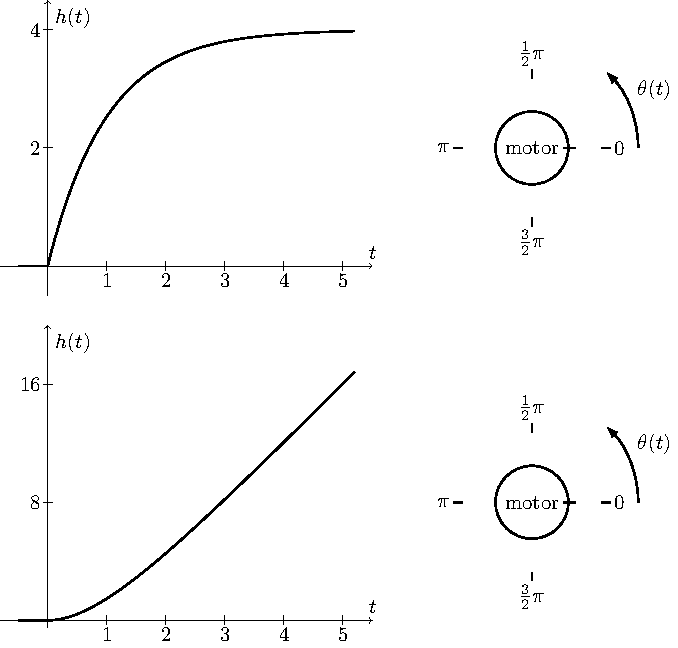
\includegraphics[page=1]{tikzfigs/dcmotorimpulseresponse}
\fi
  \caption{Impulse response (top) and step response (bottom) of a DC motor with constants $K_b= \tfrac{1}{4}$, $K_\tau = 8$ and $B=R=J=1$.} \label{fig:dcmotoranimimpulseresponse}
\end{figure}


% \section{Initial condition problems}

% The \term{unilateral Laplace transform}
% \[
% \calL_u(x,s) = \int_{0}^{\infty} x(t) e^{-st} dt
% \]



% \section{Feedback and control}\label{sec:control}

% Imagine that we would like to use a DC motor to drive an elevator that moves people between floors of a building.  Say that to move the elevator up a single floor the motor must make a single revolution, i.e., must increase it's angle by $2\pi$ radians.  As in Section~\ref{sec:direct-curr-motors-1} the equation describing the relationship between the input voltage signal and the angle of the motor is
% \[
% v = a D(\theta) + b D^2(\theta),
% \]
% where $a = \tfrac{RB}{K_\tau} + K_b$ and $b=\tfrac{RJ}{K_\tau}$ where $R,B,K_\tau,K_b,$ and $J$ and are related to components of the motor as described in Section~\ref{sec:direct-curr-motors}.

% Assume for the moment that the motor parameters satisfy $a=2$ and $b=3$.  Using the differential equation, we can design an input voltage signal that will make the motor perform a single revolution by $2\pi$, i.e., move the elevator up by one floor.  For example, put
% \begin{equation}\label{eq:thetaelevatordesigned}
% \theta(t) = \begin{cases}
% 0 & t \leq 0 \\
% \pi - \pi\cos(t) & 0 < t \leq \pi \\
% 2\pi & t > \pi.
% \end{cases}
% \end{equation}
% The input voltage signal corresponding with this signal $\theta$ is
% \begin{equation}\label{eq:velevatordesigned}
% v = 2 D(\theta) + 3 D^2(\theta) = \begin{cases}
% 0 & t \leq 0 \\
% 2\pi\sin(t) + 3\pi\cos(t)& 0 < t \leq \pi \\
% 0 & t > \pi.
% \end{cases}
% \end{equation}
% These signals are plotted in Figure~\ref{fig:designedelevatoropenloop}.  This input voltage signal drives the motor to perform precisely a rotation by $2\pi$, corresponding with the elevator moving up by a single floor.  

% This signal $v$ has been designed specifically for the case when $a = 2$ and $b=3$.  Say that the elevator is expected to carry up to a maximum of 6 people.  The inertial load $J$ on the motor varies with the number of passengers.  Also, it is found that during periods of consistent use the motor heats up causing the internal resistance of the motor $R$ to change.  After these effects are taken into account it is found that the coefficients $a$ and $b$ in the differential equation describing the motor can vary within the ranges $1 \leq a \leq 3$ and $1 \leq b \leq 7$.  These changes affect our ability to control the elevator.  From~\eqref{eq:impulseresponseDCmotor}, the impulse response of the motor is
% \[
% h(t) =  \tfrac{1}{a} u(t)\big( 1 - e^{-a t/b}\big).
% \]
% For any given $a$ and $b$ the reponse of the motor to input voltage $v$ from~\eqref{eq:velevatordesigned} is 
% \[
% \theta_{a,b}(t) =  h * v = \int_{-\infty}^{\infty} h(\tau) v(t - \tau) d\tau,
% \]
% and this can be shown (Exercise~\eqref{exer:elevatorgeneralequation}) to take the from
% \begin{equation}\label{eq:generalequationelevator}
% \theta_{a,b}(t) = \begin{cases}
% 0 & t \leq 0 \\
% \frac{2\pi}{a} + A e^{-at/b} +  B\cos(t) +  C \sin(t) & 0 < t \leq \pi\\
% \frac{4\pi}{a} +  A e^{-at/b} (1+e^{a\pi/b}) & t > \pi,
% \end{cases}
% \end{equation}
% where 
% \[
% A = \frac{\pi(3a - 2b)b}{a(a^2+b^2)}, \qquad  B =  -\frac{\pi(2a +3b)}{a^2+b^2}, \qquad C = \frac{a}{b}A.
% \]

% Figure~\ref{eq:motorelevatoropenloop} plots the motor angle signal $\theta_{a,b}$ for pairs $(a,b) = (2,3)$, $(4,3)$, $(2,1)$, $(2,7)$, $(1.5,3)$, $(3,3)$.

% \begin{figure}[tp]
%   \centering
%   \defaultanimation{tikzfigs/designedperfectopenloopmotor}  
%   \animategraphics[autoplay,loop,every=\every]{\defaultframerate}{tikzfigs/designedperfectopenloopmotor}{}{}
%   \caption{Motion of DC motor with input voltage~\eqref{eq:velevatordesigned} when $a=2$ and $b=3$.}\label{fig:designedelevatoropenloop}
% \end{figure}

% \begin{figure}[p]
%   \centering
%   \defaultanimation{tikzfigs/openloopdcmotors}  
%   \animategraphics[autoplay,loop,every=\every]{\defaultframerate}{tikzfigs/openloopdcmotors}{}{}
%   \caption{Motion of DC motor with input voltage~\eqref{eq:velevatordesigned} for cofficient pairs $(a,b) = (2,3)$, $(4,3)$, $(2,1)$, $(2,7)$, $(1.5,3)$, $(3,3)$.}\label{eq:motorelevatoropenloop}
% \end{figure}


% %The DC motor is not stable.  Let $H$ be the system that maps input voltage $x$ to motor angle $y$.  Assume we are able to measure the angle of the motor $\theta$.  Consider the system that results from applying a system $G$ to $\theta$ and adding this to the input voltage signal $x$ before it is input to the motor.  This is depicted in Figure~\ref{blockdiag:feedback}.  The input voltage and motor angle now satisfy

% Let $H$ be a linear shift-invariant system.  Assume that the signal $y$ output from $H$ can be measured.  Consider the system that results from applying a system $G$ to $y$ and adding the resopnse to an input signal $x$, that is then input to the system $H$.  This is depicted in Figure~\ref{blockdiag:feedback}. 
% \[
% y = H\big( x + G(y) \big) = H(x) + H\big(G(y)\big).
% \]
% Taking Laplace tranforms on both sides
% \[
% \calL(y) = \lambda(H)\calL(x) + \lambda(H)\lambda(G)\calL(y)
% \]
% and we find a system that maps $x$ to $y$, say $F$, now has transfer function
% \[
% \lambda(F) = \frac{\calL(y)}{\calL(x)} = \frac{\lambda(H)}{1 - \lambda(H)\lambda(G)}.
% \]
% The system $H$ might not have desirable properties, but if $G$ is appropriately chosen, the system $F$ might have more desirable properties.




% \begin{figure}
%   \centering
%   \begin{tikzpicture}[node distance=1.5cm,auto,>=latex']

%     \node [dspnodeopen] (x) [label=left:$x$] {};
%     \node[dspadder] (adder) [right of=x] {};
%     \node[coordinate] (belowadder) [below of=adder] {};
%     \node [dspsquare] (H) [right of=adder] {$H$};    
%     \node[coordinate] (feedbackconnector) [right of=H] {};
%     \node[coordinate] (belowfeedbackconnector) [below of=feedbackconnector] {};
%     \node [dspnodeopen] (y) [right of=feedbackconnector,label=right:$y$] {};
%     \node [dspsquare] (G) [below of=H] {$G$}; 

%     \draw[dspflow] (x) -- (adder);
%     \draw[dspflow] (adder) -- (H);
%     \draw[dspflow] (H) -- (feedbackconnector);
%     \draw[dspflow] (feedbackconnector) -- (y);
%     \draw[dspflow] (feedbackconnector) -- (belowfeedbackconnector);
%     \draw[thick,line cap=round] (belowfeedbackconnector) -- (G);
%     \draw[thick,line cap=round] (G) -- (belowadder);
%     \draw[dspflow] (belowadder) -- (adder);

%     \node (F) at (3,-0.75) [draw,thick,dashed,minimum width=3.9cm,minimum height=3cm,label=above:$F$] {};

%   \end{tikzpicture}
%   \caption{Feedback block diagram.  The system $F$ satisfies $y = H\big(x + G(y)\big)$.}\label{blockdiag:feedback}
% \end{figure}


%%% Local Variables: 
%%% mode: latex
%%% TeX-master: "main.tex"
%%% End: 